%!TEX root = ../agi_mfws414ali.tex
\section*{Anhang}
\addcontentsline{toc}{section}{Anhang}
\fancyhead[R]{Anhang}

\anhangsverzeichnis

\anhang{Messreihen - Einzelspieler} \label{appendix:testSingle}
\subanhang{Einzelspieler: LipkeAnts}
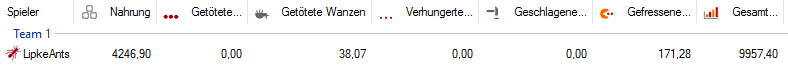
\includegraphics[scale=.7]{img/LipkeAnts.PNG}

\subanhang{Einzelspieler: aTomApfelmeisen}
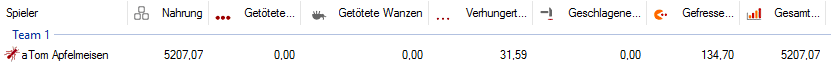
\includegraphics[scale=.7]{img/aTomApfelmeisen.PNG}

\subanhang{Einzelspieler: aTomGruppenmeisen}
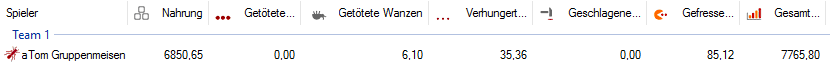
\includegraphics[scale=.7]{img/aTomGruppenmeisen.PNG}

\subanhang{Einzelspieler: aTomKampfmeisen}
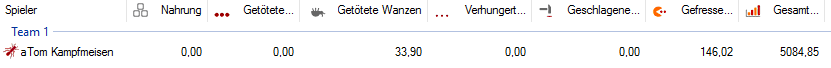
\includegraphics[scale=.7]{img/aTomKampfmeisen.PNG}

\subanhang{Einzelspieler: aTomZuckermeisen}
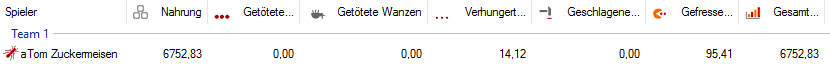
\includegraphics[scale=.7]{img/aTomZuckermeisen.PNG}

\anhang{Messreihen - Mehrspieler} \label{appendix:testMulti}
\subanhang{Mehrspieler: LipkeAnts - aTomApfelmeisen}
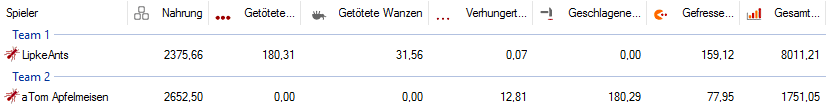
\includegraphics[scale=.7]{img/LipkeAnts_aTomApfelmeisen.PNG}

\subanhang{Mehrspieler: LipkeAnts - aTomGruppenmeisen}
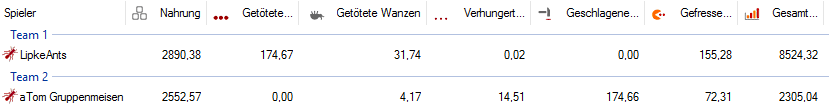
\includegraphics[scale=.7]{img/LipkeAnts_aTomGruppenmeisen.PNG}

\subanhang{Mehrspieler: LipkeAnts - aTomKampfmeisen}
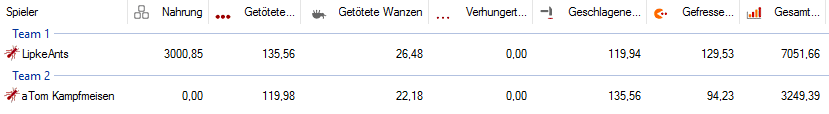
\includegraphics[scale=.7]{img/LipkeAnts_aTomKampfmeisen.PNG}

\subanhang{Mehrspieler: LipkeAnts - aTomZuckermeisen}
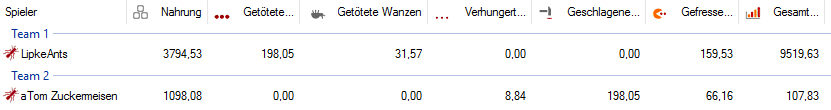
\includegraphics[scale=.7]{img/LipkeAnts_aTomZuckermeisen.PNG}

\pagebreak
\anhang{Quellcode des AntMe!-Volkes \textit{LipkeAnts}}
\lstinputlisting[language=C, frame=single, numbers=left]{code/LipkeAntsClass.cs}

\pagebreak
\anhang{Latex Quellcode}

\subanhang{Masterdatei}
\lstinputlisting[language=TeX, frame=single, numbers=left]{agi_mfws414ali.tex}

\pagebreak
\subanhang{Config}
\lstinputlisting[language=TeX, frame=single, numbers=left]{config/Config.tex}

\subanhang{Titelseite}
\lstinputlisting[language=TeX, frame=single, numbers=left]{chapter/Titelseite.tex}

\subanhang{Kapitel 1 - Einleitung}
\lstinputlisting[language=TeX, frame=single, numbers=left]{chapter/Einleitung.tex}

\subanhang{Kapitel 2 - Elementares Konzept und Randbedingungen}
\lstinputlisting[language=TeX, frame=single, numbers=left]{chapter/Elementares_Konzept.tex}

\subanhang{Kapitel 3 - Dokumentation}
\lstinputlisting[language=TeX, frame=single, numbers=left]{chapter/Dokumentation.tex}

\subanhang{Kapitel 4 - Zusammenfassung}
\lstinputlisting[language=TeX, frame=single, numbers=left]{chapter/Zusammenfassung.tex}

\subanhang{Quellenverzeichnis}
\lstinputlisting[language=TeX, frame=single, numbers=left]{chapter/Quellenverzeichnis.tex}

\subanhang{Ehrenwörtliche Erklärung}
\lstinputlisting[language=TeX, frame=single, numbers=left]{chapter/Ehrenwoertliche_Erklaerung.tex}